\documentclass{beamer}
\usepackage{graphicx} % Required for inserting images
\usepackage{german}
\usepackage{amsmath}
\usepackage{amssymb}
\usepackage{amsthm}
\usepackage{url}
\usepackage{tikz}
\usepackage[T1]{fontenc}



\newcommand{\R}{\mathbb{R}}% reele Zahlen
\newcommand{\C}{\mathbb{C}}% komplexe Zahlen
\newcommand{\Q}{\mathbb{Q}}% rationale Zahlen


\newtheorem{thm}{Satz}
\newtheorem{cor}[thm]{Korollar}
\newtheorem{lem}[thm]{Lemma}
\newtheorem{prop}[thm]{Proposition}

\title{Proseminar: Sortieralgorithmen}
\author{Maya Neudorf}
\date{\today}

\begin{document}

% Title Slide
\begin{frame}
    \titlepage
\end{frame}
\begin{frame}{Inhatltsverzeichnis}
\begin{itemize}
    \item Definition Ordnung
    \item das allgemeine Sortierproblem
    \item Sortieren durch sukzessive Auswahl
    \item Mergesort
    \item zentraler Satz zur Anzahl der Vergleiche 
    \item Quicksort
    \item Heapsort
\end{itemize}
    
\end{frame}

% First Content Slide
\begin{frame}{Ordnung Definition}
 \begin{block}{ Partielle Ordnung:}
 Sei $S$ eine Menge. Eine Relation $R \subseteq S \times S$, wenn folgende Eigenschaften gelten:
    \begin{itemize}
        \item[(a)] $(a,a) \in R$  (Reflexität);
        \item[(b)]$((a,b) \in R \wedge (b,a) \in R) \Rightarrow a=b$  (Antisymmetrie)
	\item [(c)]$((a,b \in R \wedge (b,c) \in R \Rightarrow (a,c) \in R$  (Transitivität)
    \end{itemize}
\end{block}
\begin{block}{ Totale Ordnung:}
 Eine partielle Ordnung R von S, wenn $(a,b) \in R$ oder $(b,a) \in R$ für alle $a,b \in S$ gilt 
\end{block}
\end{frame}
\begin{frame}{Das allgemeine Sortierproblem}
\begin{block}{Input}
eine endliche Menge $S$ mit einer partitiellen Ordnung $\preceq$
\end{block}
\begin{block}{Ausgabe}
Berechne eine Bijektion $f \colon \{1,\dots,n\} \to S$ mit $f(j) \not\preceq f(i)$ für alle $1\le i<j \le n$ (eine sortierte Liste)
\end{block}
\begin{block}{naives Verfahren}
Alle $n!$ Permutationen ausprobieren und testen ob für alle $n(n-1)/2$ Paare $(i,j) $$  f(j) \not\le f(i)$ gilt.
\end{block}
\end{frame}
\begin{frame}{Sortieren durch sukzessive Auswahl}
\begin{block}{Eingabe:} eine Menge $S = \{s_1, \dots, s_n\}$; eine partielle Ordnung $\preceq $ auf $S$ 
\end{block}
    \begin{block}{Ausgabe:} eine Bijektion $f : \{1, \dots, n\} \to S$ mit $f(j) \not\preceq f(i)$ für alle $1 \leq i < j \leq n$.\\
    \textbf{for} {$i \leftarrow 1$ \textbf{to} $n$} \textbf{do} $f(i) \leftarrow s_i$\\
    \textbf{for} {$i \leftarrow 1$ \textbf{to} $n$}\\
        \textbf{for} {$j \leftarrow i$ \textbf{to} $n$}\\
            \textbf{if} {$f(j) \le f(i)$} 
                \textbf{then swap}($f(i), f(j)$)\\
            \textbf{output} $f$

    \end{block}

\end{frame}
\begin{frame}
\begin{block}{Beweis für Korrektheit des Algorithmus}
Wir zeigen, dass für alle $1 \le i \le j \le n$  nach Iteration (i,j) folgendes gilt:
\begin{itemize}
\item[(a)]$f(k) \not \preceq f(i) $ für alle $1 \le h <i$ und $h<k\le n$ (vor i ist die Liste sortiert)
\item[(b)]$f(k) \not \preceq ,f(i)$ für alle $i<k \le j$ (i ist kleiner als alles rechts davon)
\end{itemize}
Für b)  1.Fall $f(j)\not \preceq f(i)$: es wird nichts getauscht. b) gilt also
	2.Fall:$ f(j) \preceq f(i)$, betrachte Index $k$ mit $i<k \le j$: für $j=k$ gilt wegen der Antisymmetrie b) nach dem swap-Befehl.
für $k<j$ galt zuvor $f(k)\not\preceq f(i)$ und somit $f(k) \not\preceq f(j)$. Es gilt also b).
\end{block}
\begin{block}{Die Laufzeit des Algorithmus ist $O(n^2)$.}
\end{block}
\end{frame}
\begin{frame}{Sortieren nach Schlüsseln}
\begin{block}{Input}
eine endliche Menge $S$, sowie eine Funktion $k: S \colon K$ und eine totale Ordnung auf K.
\end{block}
\begin{block}{Ausgabe}
Berechne eine Bijektion $f \colon \{1,\dots,n\} \to S$ mit $k(j) \not\preceq k(i)$ für alle $1\le i<j \le n$ (eine sortierte Liste von Schlüsseln)
\end{block}
\begin{block}{Beispiele}
Bucketsort, Insertion sort, Bubblesort
\end{block}
\end{frame}
\begin{frame}{Mergesort}
\begin{block}{Input}
eine  Menge $S=\{s_1; \cdots ;s_n \}$; eine durch Schlüssel induzierte partielle Ordnung $\preceq $ auf $S$.
\end{block}
\begin{block}{Ausgabe}
Berechne eine Bijektion $f \colon \{1,\dots,n\} \to S$ mit $f(j) \not\preceq f(i)$ für alle $1\le i<j \le n$.
\textbf{if}{$|S| > 1$}
\textbf{then} \\ \begin{itemize}
    \item  sei $S = S_1 \; \dot{\cup}\;S_2$ mit $|S_1| = \lfloor \frac{n}{2} \rfloor$ und $|S_2| =\lceil \frac{n}{2} \rceil$
\item sortiere $S_1$ und $S_2$(rekursiv mit Mergesort)
\item Verschmelze die Sortierungen von $S_1$ und $S_2$ zu Sortierung $S$.
\end{itemize}
\end{block}
\end{frame}
\begin{frame}
\begin{block}{Mergesort sortiert $n$ Elemente in der Laufzeit $O(n log n)$}
\end{block}
\begin{block}{Beweis:}
Sei $c \in \mathbb{N}$ mit $T(1) \leq c$ und 
\[
T(n) \leq T(\lfloor \tfrac{n}{2} \rfloor) + T(\lceil \tfrac{n}{2} \rceil) + cn \quad \text{für alle } n \geq 2.
\]

\textbf{Behauptung:} $T(2^k) \leq c(k+1)2^k$ für alle $k \in \mathbb{N} \cup \{0\}$.

Induktion über $k$: 
Für $k = 0$ trivial. 

Für $k \in \mathbb{N}$ gilt:
\[
T(2^k) \leq 2 \cdot T(2^{k-1}) + c 2^k \leq 2 \cdot ck 2^{k-1} + c 2^k = c(k+1)2^k.
\]

$\Rightarrow   n \in \mathbb{N}$ mit $k := \lceil \log_2 n \rceil < 1 + \log_2 n$:
\[
T(n) \leq T(2^k) \leq c(k+1)2^k < 2c(2 + \log_2 n)n = O(n \log n).
\]

\end{block}
\end{frame}
\begin{frame}{Satz}
\begin{block}{}
Jeder Sortieralgorithmus, der nur mit paarweisen Vergleichen von zwei Elementen arbeitet, benötigt zum sortieren einer n-elementigen Menge mindestens $log_2(n!)$ Vergleiche.
\end{block}
\end{frame}
\begin{frame}
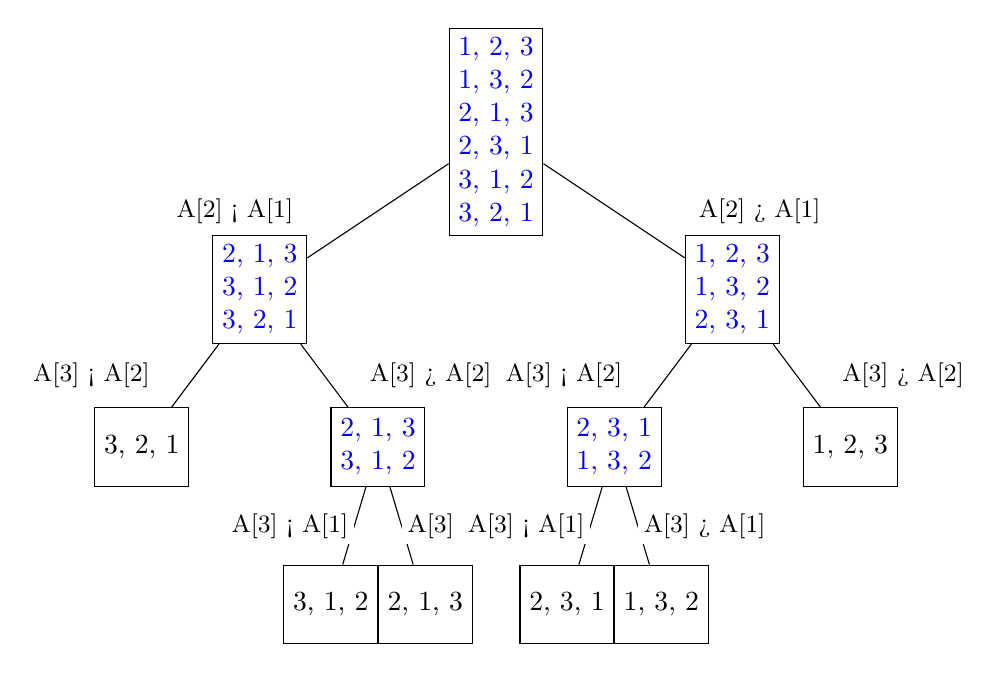
\begin{tikzpicture}[
    level distance=2cm,
    level 1/.style={sibling distance=6cm},
    level 2/.style={sibling distance=3cm},
    level 3/.style={sibling distance=1.2cm},
    box/.style={draw, rectangle, align=center, minimum height=1cm, color=blue},
    edge_label/.style={fill=white, font=\small, inner sep=2pt}
]

% Wurzelknoten
\node[box, black] (root) {\color{blue} 1, 2, 3 \\ \color{blue} 1, 3, 2 \\ \color{blue} 2, 1, 3 \\ \color{blue} 2, 3, 1 \\ \color{blue} 3, 1, 2 \\ \color{blue} 3, 2, 1}
    child {
        node[box, black] (n1) {\color{blue} 2, 1, 3 \\ \color{blue} 3, 1, 2 \\ \color{blue} 3, 2, 1}
        child {
            node[box, black] {3, 2, 1}
            edge from parent node[edge_label, left, xshift=-0.5cm] {A[3] < A[2]}
        }
        child {
            node[box, black] (n12) {\color{blue} 2, 1, 3 \\ \color{blue} 3, 1, 2}
            child {
                node[box, black] {3, 1, 2}
                edge from parent node[edge_label, left] {A[3] < A[1]}
            }
            child {
                node[box, black] {2, 1, 3}
                edge from parent node[edge_label, right] {A[3] > A[1]}
            }
            edge from parent node[edge_label, right, xshift=0.5cm] {A[3] > A[2]}
        }
        edge from parent node[edge_label, left, xshift=-1cm] {A[2] < A[1]}
    }
    child {
        node[box, black] (n2) {\color{blue} 1, 2, 3 \\ \color{blue} 1, 3, 2 \\ \color{blue} 2, 3, 1}
        child {
            node[box, black] (n21) {\color{blue} 2, 3, 1 \\ \color{blue} 1, 3, 2}
            child {
                node[box, black] {2, 3, 1}
                edge from parent node[edge_label, left] {A[3] < A[1]}
            }
            child {
                node[box, black] {1, 3, 2}
                edge from parent node[edge_label, right] {A[3] > A[1]}
            }
            edge from parent node[edge_label, left, xshift=-0.5cm] {A[3] < A[2]}
        }
        child {
            node[box, black] {1, 2, 3}
            edge from parent node[edge_label, right, xshift=0.5cm] {A[3] > A[2]}
        }
        edge from parent node[edge_label, right, xshift=1cm] {A[2] > A[1]}
    };

\end{tikzpicture}
\end{frame}
\begin{frame}
\begin{block}{Beweis:}
Gegeben: Eingabemenge $S=\{1,\cdots,n\}$ mit einer totalen Ordnung

Gesucht: einer der n! Permutationen (Blätter im Vergleichsbaum). 
Jeder Vergleich halbiert die Anzahl an möglichen Permtationen (ein Vergleich ist ein Schritt im Baum).
Ein Algorithmus braucht also $k$ Vergleiche mit $2^k\ge n! $$\Rightarrow k\ge \log_2(n!)$.

Im Allgemeinen werden mehr Vegleiche gebraucht(Beispiel n=5)
\end{block} 
\end{frame}
\begin{frame}{Quicksort}
\begin{block}{Input}
eine  Menge $S=\{s_1; \cdots ;s_n \}$; eine durch Schlüssel induzierte partielle Ordnung $\preceq $ auf $S$.
\end{block}
\begin{block}{Ausgabe}
Berechne eine Bijektion $f \colon \{1,\dots,n\} \to S$ mit $f(j) \not\preceq f(i)$ für alle $1\le i<j \le n$.\\
\textbf{if} $|S| > 1$ \textbf{then} \\\begin{itemize} \item wähle $x\in S$ beliebig
     \item $S_1 := \{s \in S \mid s \leq x\} \setminus \{x\}$
    \item$S_2 := \{s \in S \mid x \leq s\} \setminus \{x\}$
   \item $S_x := S \setminus (S_1 \cup S_2)$
    \item Sortiere $S_1$ und $S_2$ (soweit nicht leer) rekursiv mit Quicksort
    \item  Füge die sortierten Mengen $S_1$, $S_x$ und $S_2$ aneinander
    \end{itemize}
\end{block}


\end{frame}

\begin{frame}{Quicksort sortiert $n$ Elemente in der Laufzeit $O(n^2)$}
\begin{block}{Beweis}
Es exististiert ein $c\in \mathbb{N}$ mit $T(1) \leq c$.
$T(n)\leq cn + \max_{\substack{0\leq l \leq n-1}}(T(l)+T(n-1-l))
 $ für alle $n\geq 2$.
 Behauptung:$T(n)\leq cn^2 $\\
 Beweis per Induktion über n: Für $n=1$ trivial.\\
 $T(n)\leq \max_{\substack{0\leq l \leq n-1}}(cl^2+c(n-1-l)^2) = cn+ c(n-1)^2 < cn^2$
\end{block}
\begin{block}{Vorteil: es wird kein zusätzlicher temporärer Speicherplatz benötigt}
\end{block}
\end{frame}
\begin{frame}{die Wahl des x}
\begin{block}{x als erstes Element oder zufällig}
unkompliziert, für bereits sortierte Listen oder kurze Listen gut(Lauzeit:$O(n^2)$) 
\end{block}
\begin{block}{x als Median}
Median finden ist relativ aufwendig, leichteres sortieren,gut für lange Listen(Laufzeit:$O(n)$(Median ermitteln)$+O(nlog n)$ (sortieren)) 
\end{block}
\end{frame}
\begin{frame}{Der Erwartungswert der Laufzeit von Random-Quicksort für $n$ Elemente ist $O(n log(n))$}
\begin{block}{Beweis}
Es exististiert ein $c\in \mathbb{N}$ mit $\overline{T}(1) \leq c$.
$\overline{T}(n)\leq cn + \frac{1}{n} \sum_{i=1}^{n} (\overline{T}(i-1) + \overline{T}(n-i)) = cn + \frac{2}{n} \sum_{i=1}^{n-1} \overline{T}(i)
 $ für alle $n\geq 2$.
 \textbf{Behauptung:} $\overline{T}(n) < 2cn(1 + \ln n)$. \\
Wir zeigen dies per Induktion über $n$. Für $n = 1$ ist die Aussage trivial. Für $n \geq 2$ erhalten wir mit der Induktionsvoraussetzung:

\begin{align*}
\overline{T}(n) &\leq cn + \frac{2}{n} \sum_{i=1}^{n-1} 2ci(1 + \ln i) \\
&\leq cn + \frac{2c}{n} \int_{1}^{n} 2x(1 + \ln x) \, dx \\
&= cn + \frac{2c}{n} \left[ x^2(1 + \ln x) - \frac{x^2}{2} \right]_{1}^{n} \\
&= cn + 2cn(1 + \ln n) - cn - \frac{c}{n} 
&< 2cn(1 + \ln n)
\end{align*}
\end{block}
\end{frame}
\begin{frame}{Heapsort}
\begin{block}{Definition Heap}
 Ein \textbf{Heap} für eine endliche Menge $S$ mit Schlüsseln $k: S \to K$ und einer totalen Ordnung $\leq$ von $K$ ist eine Arboreszenz $A$ mit einer Bijektion $f: V(A) \to S$, so dass die Heapordnung
 
$k(f(v)) \leq k(f(w)) \quad \text{für alle } (v, w) \in E(A) $
gilt.
\end{block}
\begin{block}{}
(Ein Baum, in dem jedes Elternteil einen kleineren Wert hat als seine Kinder)
\end{block}
\begin{block}{Heapsort sortiert $n$ Elemente in der Laufzeit $O(nlog(n))$}
Der Baum ist maximal $\log_2(n)$ tief $\Rightarrow$ eine Operation kostet $O(log(n))$ und es müssen $n$ Elemnete hinzugefügt werden.
\end{block}
\end{frame}
\begin{frame}{Literaturverzeichnis}
\begin{itemize}
    \item Stefan Hougary and Jens Vygen: Algorithmische Mathematik ( 2018, Springer Spektrum)
    \item Folien zu Algorithmen und Datenstrukturen von Prof.Dr. Markus Nebel(Sose2024)
\end{itemize}
\end{frame}



\end{document}
